\begin{frame}
    \centering
    \begin{figure}[H]
        
\includegraphics[keepaspectratio, width=0.7\paperwidth, height=\paperheight]{Logos/LeeLogo}
    \end{figure}
    Informatik: Data Science und Sicherheit\\
    \textbf{Zahlensysteme} \emoji{pencil}: \textbf{Lektion 03}
\end{frame}



\begin{frame}{Stellenwertdarstellung \& $b$-adische Zahlensysteme}
\begin{itemize}
        \item Das \textcolor{red}{Dezimalsystem} hat die Basisgrössen
        $$10^0=1,\quad 10^1=10,\quad 10^2=100,\quad 10^3=1000,...$$
        \item Das \textcolor{red}{Binärsystem} hat die Basisgrössen
        $$2^0=1,\quad 2^1=2,\quad 2^2=4,\quad 2^3=8,...$$
        \item Allgemein: Das \textcolor{red}{$b$-adische System} hat die Basisgrössen
        $$b^0,\quad b^1,\quad b^2,\quad b^3,...$$
    \end{itemize}
    \rule{\textwidth}{0.4pt}
    Beispiel: Das Wort \textcolor{red}{$4605_{10}$} wird interpretiert als die Zahl
    \begin{align*}
        \textcolor{red}{4}\cdot \underbrace{10^3}_{1000} + \textcolor{red}{6}\cdot \underbrace{10^2}_{100} + \textcolor{red}{0}\cdot \underbrace{10^1}_{10} + \textcolor{red}{5}\cdot \underbrace{10^0}_{1}.
    \end{align*}
    $\rightarrow$ \tib{greedy}-Algorithmus, um Zahlen zu konvertieren
\end{frame}

\begin{frame}{Kleine Mathe-Wiederholung \emoji{nerd-face}\emoji{books}}
Wie kann man die Zahl umschreiben? $\rightarrow$ \tib{Wissenschaftliche Notation} oder \tib{Exponentialdarstellung}
\[ 10^b\cdot a\]
Beispiel:
\[500.11 = 10^2\cdot 5.0011 \]
    \begin{itemize}
        \item 
        \only<1>{$0.0003 = 10^{b}\cdot a$}
        \only<2->{$0.0003 = \underbrace{10^{-4}}_{=0.0001}\cdot 3$}
        \item
        \only<1-2>{$5'000 = 10^{b}\cdot a$}
        \only<3->{$5'000 = \underbrace{10^{3}}_{=1'000}\cdot 5$}
        \item
        \only<1-3>{$10'003.3455 = 10^{b}\cdot a$}
        \only<4->{$10'003.3455 = \underbrace{10^{4}}_{=10'000}\cdot 1.0033455$}
    \end{itemize}
\end{frame}

\begin{frame}{Stellenwertdarstellung}{Beispiel}
Frage: Wie stellen wir Kommazahlen dar?
    Z.B. \textcolor{red}{$3.4375$}\\
    \rule{\textwidth}{0.4pt}
    \only<1-4>{
    Das Wort
    \begin{align*}
        a_na_{n-1}\ldots a_1a_0.b_1b_2\ldots b_m
    \end{align*}
    entspricht definitionsgemäss der Zahl
    \begin{align*}
        a_n\cdot d^n + a_{n-1}\cdot d^{n-1}+\ldots + a_1\cdot d^1 + a_0\cdot d^0 + \\
        b_1\cdot d^{-1} + b_2\cdot d^{-2} + \ldots + b_{m-1}\cdot d^{-m-1} + b_m\cdot d^{-m} 
    \end{align*}
    \rule{\textwidth}{0.4pt}
    }
    \only<2>{
    daher haben wir, im dezimalen Zahlensystem ($d=10$):
    \begin{align*}
    \tiny
        \textcolor{red}{a_1}\cdot\underbrace{10^0}_{?} + 
        \textcolor{red}{b_1}\cdot\underbrace{10^{-1}}_{?} +
        \textcolor{red}{b_2}\cdot\underbrace{10^{-2}}_{?} +
        \textcolor{red}{b_3}\cdot\underbrace{10^{-3}}_{?} +
        \textcolor{red}{b_4}\cdot\underbrace{10^{-4}}_{?}
    \end{align*}
    }
    \only<3>{
    daher haben wir, im dezimalen Zahlensystem ($d=10$):
    \begin{align*}
    \tiny
        \textcolor{red}{a_1}\cdot\underbrace{10^0}_{1} + 
        \textcolor{red}{b_1}\cdot\underbrace{10^{-1}}_{0.1} +
        \textcolor{red}{b_2}\cdot\underbrace{10^{-2}}_{0.01} +
        \textcolor{red}{b_3}\cdot\underbrace{10^{-3}}_{0.001} +
        \textcolor{red}{b_4}\cdot\underbrace{10^{-4}}_{0.0001}
    \end{align*}
    }
    \only<4->{
    daher haben wir, im dezimalen Zahlensystem ($d=10$):
    \begin{align*}
    \tiny
        \textcolor{red}{\overbrace{3}^{a_0}}\cdot\underbrace{10^0}_{1} + 
        \textcolor{red}{\overbrace{4}^{b_1}}\cdot\underbrace{10^{-1}}_{0.1} +
        \textcolor{red}{\overbrace{3}^{b_2}}\cdot\underbrace{10^{-2}}_{0.01} +
        \textcolor{red}{\overbrace{7}^{b_3}}\cdot\underbrace{10^{-3}}_{0.001} +
        \textcolor{red}{\overbrace{5}^{b_4}}\cdot\underbrace{10^{-4}}_{0.0001}
    \end{align*}
    }
    \only<5-8>{
    Im binären Zahlensystem ($d=2$):
    }
    \only<5>{
    \begin{align*}
    \tiny
        \textcolor{red}{a_1}\cdot\underbrace{2^1}_{?} + 
        \textcolor{red}{a_0}\cdot\underbrace{2^0}_{?} + 
        \textcolor{red}{b_1}\cdot\underbrace{2^{-1}}_{?} +
        \textcolor{red}{b_2}\cdot\underbrace{2^{-2}}_{?} +
        \textcolor{red}{b_3}\cdot\underbrace{2^{-3}}_{?} +
        \textcolor{red}{b_4}\cdot\underbrace{2^{-4}}_{?}
    \end{align*}
    }
    \only<6>{
    \begin{align*}
    \tiny
        \textcolor{red}{a_1}\cdot\underbrace{2^1}_{2} + 
        \textcolor{red}{a_0}\cdot\underbrace{2^0}_{1} + 
        \textcolor{red}{b_1}\cdot\underbrace{2^{-1}}_{1/2=0.5} +
        \textcolor{red}{b_2}\cdot\underbrace{2^{-2}}_{1/4=0.25} +
        \textcolor{red}{b_3}\cdot\underbrace{2^{-3}}_{1/8=0.125} +
        \textcolor{red}{b_4}\cdot\underbrace{2^{-4}}_{0.0625}
    \end{align*}
    }
    \only<7->{
    \begin{align*}
    \tiny
        \textcolor{red}{1}\cdot\underbrace{2^1}_{2} + 
        \textcolor{red}{1}\cdot\underbrace{2^0}_{1} + 
        \textcolor{red}{0}\cdot\underbrace{2^{-1}}_{1/2=0.5} +
        \textcolor{red}{1}\cdot\underbrace{2^{-2}}_{1/4=0.25} +
        \textcolor{red}{1}\cdot\underbrace{2^{-3}}_{1/8=0.125} +
        \textcolor{red}{1}\cdot\underbrace{2^{-4}}_{0.0625}
    \end{align*}
    }
    \only<8>{
    \rule{\textwidth}{0.4pt}
    Wir wissen nun also, dass \textcolor{red}{$3.4375_{10}=11.0111_2$}
    }
    
\end{frame}

\begin{frame}{Stellenwertdarstellung}{Verallgemeinerung}
    \rule{\textwidth}{0.4pt}
    Seien $a_n,a_{n-1},\ldots,a_1,a_0$ natürliche Zahlen. Dann stellt das Wort
    \begin{align*}
        a_na_{n-1}\ldots a_1a_0
    \end{align*}
    (definitionsgemäss) die Ganzzahl
    \begin{align*}
        a_n\cdot d^n + a_{n-1}\cdot d^{n-1}+\ldots + a_1\cdot d^1 + a_0\cdot d^0
    \end{align*}
    im $d$-adischen Zahlensystem dar. 
    \rule{\textwidth}{0.4pt}
    Eine Nachkommazahl wird dargestellt wie folgt:
    \begin{align*}
        a_na_{n-1}\ldots a_1a_0.b_1b_2\ldots b_m
    \end{align*}
    und entspricht definitionsgemäss der Zahl
    \begin{align*}
        a_n\cdot d^n + a_{n-1}\cdot d^{n-1}+\ldots + a_1\cdot d^1 + a_0\cdot d^0 + \\
        b_1\cdot d^{-1} + b_2\cdot d^{-2} + \ldots + b_{m-1}\cdot d^{-m-1} + b_m\cdot d^{-m} 
    \end{align*}
\end{frame}

\begin{frame}{Stellenwertdarstellung von Kommazahlen}
Einige Überlegungen
\begin{itemize}
    \item Je nach Kommazahl finden müssen wir im binären System weit suchen gehen, bis wir die Zahl korrekt abgebildet haben
    \item Wie präzise sollen / können wir Zahlen abbilden?
\end{itemize}
\end{frame}

\begin{frame}{Übungen}
\begin{itemize}
    \item Arbeiten Sie weiter an den Aufgaben von letztem Mal
    \begin{itemize}
        \item (Auffrischung) Lesen Sie ``Neue Konzepte und Begriffe'' auf S. 14.
        \item Lösen Sie Aufgabe 1.11 (Hilfestellung: im 5-adischen Zahlensystem gibt es nur die Ziffern $\{0,1,2,3,4\}$)
        \item Lesen Sie Beispiel 1.2 (Transformation von Zahlendarstellungen) und lösen Sie danach die Aufgabe 1.12.
    \end{itemize}
    \item (Auffrischung) Lesen Sie ``Neue Konzepte und Begriffe'' auf S. 24.
    \item 1.28 a und b
    \item Helfen Sie anderen!
\end{itemize}
\end{frame}

\begin{frame}{Anhang (optional)}
\end{frame}

\begin{frame}{Stellenwertdarstellung von Kommazahlen}
Präzision von Kommazahlen (Übung 1.31)
\begin{itemize}[<+->]
    \item Angenommen, wir haben 20 bits zur Verfügung und wollen Zahlen in einem Intervall von $[0, 1000)$ abspeichern, was könnten wir tun?
    \item Wir haben 20 bits zur Verfügung, also können wir $2^{20}$ unterschiedliche Zahlen modellieren (ca. $1\text{\textquotesingle}000\text{\textquotesingle}000)$. 
    \item Problem: es gibt unendlich viele Zahlen zwischen $0$ und $1000$...
    \item Erste Lösungsidee: Wir teilen das Intervall $[0,1000)$ in $1\text{\textquotesingle}000\text{\textquotesingle}000$ gleich grosse Unter-Intervalle auf (also Schritte von $0.001$, denn $0.001\cdot1000=1\text{\textquotesingle} 000\text{\textquotesingle}000$).
    \item Jede Zahl $i$ stellen wir durch den Mittelwert des i-ten Intervalls dar.
    \item \textbf{Beispiel}:
    \begin{itemize}
        \item Alle Zahlen zwischen $[0.001, 0.002)$ werden durch 0.0015 dargestellt (=Mittelwert)
        \item Alle Zahlen zwischen $[999.999, 1000)$ werden durch 999.9995 dargestellt (=Mittelwert)
    \end{itemize}
    \item Somit beträgt der absolute Fehler jeder Zahl maximal 0.0005.
\end{itemize}
\end{frame}

\begin{frame}{Stellenwertdarstellung von Kommazahlen}

\begin{itemize}[<+->]
        \item \tib{Problem}: Der relative Darstellungsfehler kann riesig sein.
            \tiny$$
            \text{Relativer Darstellungsfehler} = \frac{\abs{\text{Wert der Darstellung - Zahl}}}{\text{Zahl}}
            $$
            \normalsize
        \item Wert der Darstellung: 0.0015, echte Zahl: 0.001.\\
        \tiny$$
        \frac{\overbrace{\abs{0.0015 - 0.001}}^{\textcolor{red}{=0.0005}}}{0.001} = \text{50\%!}
        $$
        \item Wert der Darstellung: 999.9995, echte Zahl: 999.999.\\
        \tiny$$
        \frac{\overbrace{\abs{999.9995 - 999.999}}^{\textcolor{red}{=0.0005}}}{999.999} = \text{ca. 0.00005\%!}
        $$\normalsize
        \item Allgemein sehen wir, dass der relative Fehler in diesem Fall lediglich von der Zahl abhängt:
        $$\tiny
                \text{Relativer Darstellungsfehler} = \frac{\overbrace{\textcolor{red}{0.0005}}^{\text{Absoluter Darstellungsfehler}}}{\text{Zahl}}
        \normalsize$$
        \item Wir möchten aber unabhängig von der Zahl einigermassen genau rechnen können...

\end{itemize}
\end{frame}

\begin{frame}{Lösungsansatz}
% Basiert auf Übunge 1.32
Weitere Illustration (20 bits):
\begin{itemize}
\tiny
    \item $\textcolor{red}{110111001001011.001 }\textcolor{blue}{01}_2$
    \item $\textcolor{red}{1101110.010}\textcolor{blue}{0101100101}_2$
    \item $\textcolor{red}{11.011}\textcolor{blue}{100100101100101}_2$
\end{itemize}\normalsize
Der \textcolor{red}{rote} Teil ist mit dem obigen Ansatz \enquote{präzise} dargestellt, dar \textcolor{blue}{blaue} nicht. Erkennen Sie das Problem dieses Ansatzes?

\begin{itemize}
    \item Wie wir intuitiv sehen, müssen lange Zahlen gar nicht so genau sein. Bei einer Zahl wie ``1'000'000'000'' (eine Milliarde) ist es weniger wichtig, sie auf mehrere Nachkommastellen genau abzubilden, als bei einer Zahl wie ``0.0034551''. 
    \item Wenn wir eine ähnliche relative Genauigkeit für Zahlen unterschiedlicher Grössenordnungen wollen, müssen wir für kleinere Zahlen ``genauer'' sein als für grosse.
    \item Analogie: \emoji{bread}
    \begin{itemize}
        \item \emoji{carpentry-saw} Dicke Stücke können wir einer stumpfen Säge schneiden 
        \item \emoji{knife} Für hauchdünne Stücke brauchen wir ein fein geschliffenes Messer (Aufteilung des Brotes in feinere Stücke / ``Intervalle'')
    \end{itemize}
\end{itemize}
\end{frame}

\begin{frame}{Lösungsansatz (s. Übung 1.32)}
\rule{\textwidth}{0.4pt}
\begin{itemize}
    \item \tib{Lösungsidee}: Statt die Intervalle immer gleich gross zu machen, machen die Unterteilung feiner für kleinere Zahlen, und grösser für grössere Zahlen
\end{itemize}\rule{\textwidth}{0.4pt}\\
\only<2->{Betrachten Sie folgende Zahlen. Wie lassen sich diese Zahlen neu schreiben, um ähnliche Genauigkeit beim Abspeichern zu haben?
    \begin{enumerate}
        \item 1003030401.003 \only<3->{\textcolor{red}{$\rightarrow 10^9\cdot1.003030401003$}}
        \item 34034.11100345 \only<3->{\textcolor{red}{$\rightarrow 10^4\cdot3.403411100345$}}
        \item 9.349995613496 \only<3->{\textcolor{red}{$\rightarrow 10^0\cdot9.349995613496$}}
    \end{enumerate}}
    \only<3->{\rightarrow \tib{Normalisierte (wissenschaftliche) Darstellung}}
\end{frame}
\begin{frame}{Lösungsansatz (s. Übung 1.32)}
\begin{itemize}[<+->]
    \item Angenommen, wir wollen Zahlen zwischen 0 und 10 darstellen. Wir sagen, dass Zahlen kleiner als $10^{-31}$ (also $< 0.000\ldots 0001$) als 0 dargestellt werden.
    \item Wir haben für also $32 = 2^5$ Intervalle bezüglich 10er-Potenzen:
    \scriptsize\begin{align*}
        =&[10^{-31}, 10^{-30}),&[10^{-30}, 10^{-29}),&...,&\underbrace{[10^{-2}, 10^{-1})}_{=[0.01, 0.1)},&\underbrace{[10^{-1}, 10^0)}_{=[0.1, 1)},& \underbrace{[10^0, 10^1)}_{=[1, 10)}&
    \end{align*}\normalsize
    \item Allgemein schreiben wir ein Intervall als $[10^i, 10^{i+1})$.
    \item Wir teilen jedes Intervall in gleich viele Unter-Intervalle auf, z.B. in Schritten von $0.01\cdot 10^i$ (d.h. je 900 Unter-Intervalle pro Intervall)\only<4->{\footnote{Die Unter-Intervalle des grössten Intervalls sind beispielsweise: $[1.00, 1.01), [1.01, 1.02), [1.02, 1.03), ..., [9.98, 9.99), [9.99, 10.00)$}}. Dann beträgt der relative Fehler immer $\frac{0.005\cdot 10^i}{10^i}=0.005$ und ist somit nun unabhängig von der Zahl!
    \item Umsetzung im Computer:
    \begin{figure}[H]
        \centering
        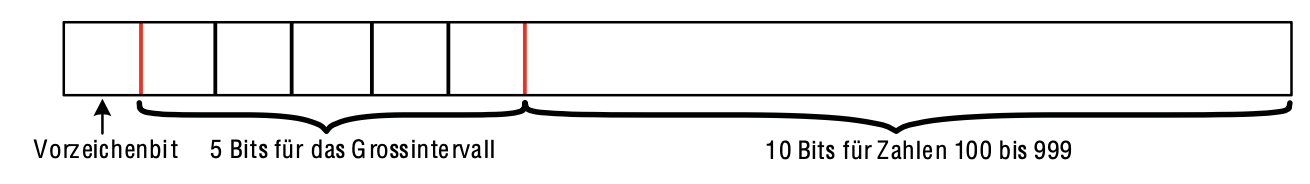
\includegraphics[keepaspectratio, width=0.75\paperwidth, height=\paperheight]{Grundlagen_Info/01_TheoretischeInformatik/Figures/4-ex132.png}
    \end{figure}
\end{itemize}
\end{frame}

\begin{frame}{Übungen}
\begin{itemize}
    \item (Optional) lesen Sie die Lösungen von Übung 1.32
    \item Lesen Sie Beispiel 1.5
    \item 1.33
\end{itemize}
\end{frame}